%%%%%%%%%%%%%%%%%%%%%%%%%%%%%%%%%%%%%%%%%
% Simple Sectioned Essay Template
% LaTeX Template
%
% This template has been downloaded from:
% http://www.latextemplates.com
%
% Note:
% The \lipsum[#] commands throughout this template generate dummy text
% to fill the template out. These commands should all be removed when 
% writing essay content.
%
%%%%%%%%%%%%%%%%%%%%%%%%%%%%%%%%%%%%%%%%%

%----------------------------------------------------------------------------------------
%	PACKAGES AND OTHER DOCUMENT CONFIGURATIONS
%----------------------------------------------------------------------------------------

\documentclass[12pt]{article} % Default font size is 12pt, it can be changed here

\usepackage{geometry} % Required to change the page size to A4
\geometry{a4paper, left={40mm}, right={40mm}, top={25mm}, bottom={25mm},includehead,includefoot} % Set the page size to be A4 as opposed to the default US Letter

\usepackage{graphicx} % Required for including pictures

\usepackage{float} % Allows putting an [H] in \begin{figure} to specify the exact location of the figure
\usepackage{wrapfig} % Allows in-line images such as the example fish picture

\usepackage{lipsum} % Used for inserting dummy 'Lorem ipsum' text into the template

\usepackage{amsfonts}

\usepackage{listings}
\usepackage{hyphenat}
\usepackage{hyperref}

\usepackage{xcolor}
\hypersetup{
    colorlinks,
    linkcolor={red!50!black},
    citecolor={blue!50!black},
    urlcolor={blue!80!black}
}

\usepackage[sorting=none]{biblatex}
\addbibresource{bibliografia.bib}

% ---------------------------------------------------------------------------------------
%	TIPOGRAFÍA
% ---------------------------------------------------------------------------------------

\usepackage[no-math]{fontspec}
\setmainfont[
	Path=./../fuentes/, 
	UprightFont=* Regular, 
	ItalicFont=* Italic,
	BoldFont=* Bold,
  	BoldItalicFont=* Bold Italic,
]{Equity Text A}
\setsansfont[
	Path=./../fuentes/, 
	UprightFont=* Regular, 
	ItalicFont=* Italic,
	BoldFont=* Bold,
  	BoldItalicFont=* Bold Italic,
]{Concourse T3}
\setmonofont[
	Path=./../fuentes/, 
	UprightFont=* Regular, 
	%ItalicFont=* Italic,
	%BoldFont=* Bold,
  	%BoldItalicFont=* Bold Italic,
  	SizeFeatures={Size=10.5},
]{Iosevka}

\usepackage[math-style=TeX]{unicode-math}
%\setmathfont{XITS Math}
\setmathfont[Path=./../fuentes/]{XITS Math}
\setmathfont[
	Path=./../fuentes/,
	range=up/{latin,Latin, num},
]{Equity Text A Regular}
\setmathfont[
	Path=./../fuentes/,
	range=it/{latin,Latin},
]{Equity Text A Italic}
\setoperatorfont\symup

\defaultfontfeatures{Ligatures=TeX,Numbers=Lining}


% ---------------------------------------------------------------------------------------
% 	CONFIGURACIÓN DEL ÍNDICE
% ---------------------------------------------------------------------------------------

\usepackage{titletoc}

\contentsmargin[0cm]{0cm}
\titlecontents{chapter}[0em]{\vskip12pt\bfseries\sffamily}
{\thecontentslabel\enspace}
{\hspace{1.05em}}
{ \hfill\contentspage}[\vskip 6pt]

\titlecontents{section}[1em]{\sffamily}
{\thecontentslabel\enspace}
{}
{\titlerule*[1pc]{.}\quad\contentspage}[\vskip 4pt]

\titlecontents{subsection}[2em]{\sffamily}
{\thecontentslabel\enspace}
{}
{\titlerule*[1pc]{.}\quad\contentspage}[\vskip 3pt]

\titlecontents{subsubsection}[4em]{\sffamily}
{\thecontentslabel\enspace}
{}
{\titlerule*[1pc]{.}\quad\contentspage}[\vskip 3pt]

\usepackage{etoolbox}
\pretocmd{\contentsname}{\sffamily}{}{}

% ---------------------------------------------------------------------------
% 	TÍTULOS DE PARTES Y SECCIONES
% ---------------------------------------------------------------------------

\usepackage{titlesec}

% Estilo de los títulos de las partes
\titleformat{\part}[hang]{\Huge\bfseries\sffamily}{\thepart\hspace{20pt}\textcolor{500}{|}\hspace{20pt}}{0pt}{\Huge\bfseries}
\titlespacing*{\part}{0cm}{-2em}{2em}[0pt]

% Reiniciamos el contador de secciones entre partes (opcional)
\makeatletter
\@addtoreset{section}{part}
\makeatother

% Estilo de los títulos de las secciones, subsecciones y subsubsecciones
\titleformat{\section}
  {\LARGE\bfseries\sffamily}{\thesection}{0.5em}{}

\titleformat{\subsection}
  {\Large\sffamily}{\thesubsection}{0.25em}{}

\titleformat{\subsubsection}
  {\large\sffamily}{\thesubsubsection}{0.25em}{}

 \usepackage[spanish]{babel}

\linespread{1.3} % Line spacing
\setlength{\parskip}{9pt}

\usepackage[bottom]{footmisc}

\renewcommand*\footnoterule{}

%----------------------------------------------------------------------------------------
%	CABECERAS Y PIES DE PÁGINA
%----------------------------------------------------------------------------------------

\usepackage{fancyhdr}
 
\pagestyle{fancy}
\fancyhf{}
\rfoot{\sffamily Página \thepage\ de \pageref{LastPage}}
\lfoot{\sffamily La web distribuida: el protocolo IPFS}

\renewcommand{\headrulewidth}{0pt}
\renewcommand{\footrulewidth}{0.5pt}

\usepackage{lastpage}

\setlength\parindent{0pt} % Uncomment to remove all indentation from paragraphs

\graphicspath{{Pictures/}} % Specifies the directory where pictures are stored

\usepackage[font=sf]{caption}

\begin{document}

%----------------------------------------------------------------------------------------
%	PÁGINA DEL TÍTULO
%----------------------------------------------------------------------------------------

\begin{titlepage}
\sffamily

\newcommand{\HRule}{\rule{\linewidth}{0.5mm}} % Defines a new command for the horizontal lines, change thickness here

\center % Center everything on the page

\textsc{\LARGE Universidad de Granada}\\[1.5cm] % Name of your university/college
\textsc{\Large Doble Grado en Ingeniería Informática y Matemáticas}\\[0.5cm] % Major heading such as course name
\textsc{\large Fundamentos de Redes}\\[0.5cm] % Minor heading such as course title

\HRule \\[1cm]
{ \huge \bfseries La web distribuida: el protocolo IPFS}\\[0.4cm] % Title of your document
\HRule \\[1.5cm]

\begin{minipage}{0.4\textwidth}
\begin{flushleft} \large
\emph{Autores:}\\
José María Martín Luque\\
Adolfo Soto Werner % Your name
\end{flushleft}
\end{minipage}
~
\begin{minipage}{0.4\textwidth}
\begin{flushright} \large
\emph{Profesor:} \\
Antonio Ruiz Moya\\ % Supervisor's Name
\hfill\\
\end{flushright}
\end{minipage}\\[4cm]

{\large \today}\\[3cm] % Date, change the \today to a set date if you want to be precise

%\includegraphics{Logo}\\[1cm] % Include a department/university logo - this will require the graphicx package

\vfill % Fill the rest of the page with whitespace

\end{titlepage}

%----------------------------------------------------------------------------------------
%	ÍNDICE
%----------------------------------------------------------------------------------------

\tableofcontents % Include a table of contents

\newpage % Begins the essay on a new page instead of on the same page as the table of contents 

%----------------------------------------------------------------------------------------
%	INTRODUCTION
%----------------------------------------------------------------------------------------

\section*{Introducción}

El Protocolo de transferencia de hipertexto (HTTP por sus siglas en inglés) es uno de los protocolos fundamentales de Internet. El desarrollo de HTTP comenzó en 1989 en el CERN por parte de Tim Berners-Lee. El desarrollo de un estándar fue un trabajo colaborativo entre el Grupo de Trabajo de Ingeniería de Internet (Internet Engineering Task Force, IETF) y el Consorcio WWW (World Wide Web Consortium, W3C), proceso que culminó con la publicación de una serie de \textit{Request for Comments} (RFCs)\footnote{Los RFCs son un tipo de documentos técnicos del IETF que datallan técnicamente diversos aspectos del funcionamiento de Internet y otros protocolos.}. La primera definición de \texttt{HTTP/1.1}, la versión de HTTP más utilizada, apareció en el RFC 2068 de 1997. 

Estamos hablando por tanto de un protocolo cuyo diseño comenzó hace más de 25 años. En aquel momento era inimaginable pensar que la tecnología que se estaba desarrollando fuese a ser usada por miles de millones de personas (3.885.567.619 a nivel mundial según las últimas estadísticas\cite{internet-world-stats} de junio de 2017) ni se esperaba que tuviese tal repercusión sobre nuestras vidas. HTTP ha simplificado y facilitado la transmisión de información a nivel mundial. Gracias a ello hemos avanzado hacia una sociedad conectada donde la información y la cultura fluye libremente.

Pero como es de esperar, un protocolo que no fue diseñado con la visión del mundo actual presenta una serie de problemas a resolver. La intención de este trabajo es mostrar las deficiencias de HTTP y explorar una alternativa a la web actual, la web distribuida y el protocolo IPFS.

\newpage


%----------------------------------------------------------------------------------------
%	CONTENIDO
%----------------------------------------------------------------------------------------

\section{Problemas de HTTP} % (fold)
\label{sec:problemas_de_http}

\subsection{Fragilidad} % (fold)
\label{sub:fragilidad}

\begin{figure}[h]
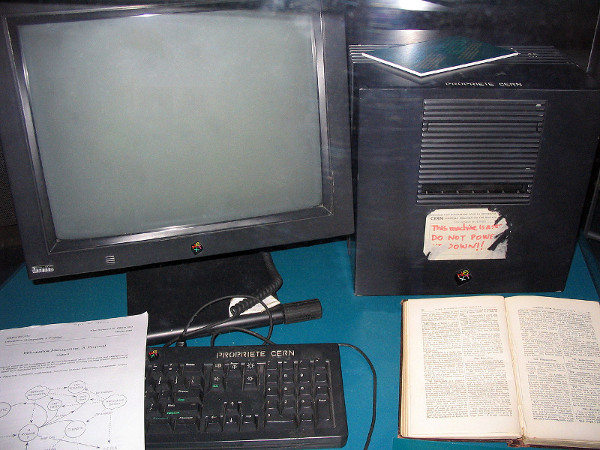
\includegraphics[width=\textwidth]{first-web-server}
\caption{Primer servidor de HTTP del mundo. Se trata del ordenador personal de Tim Berners-Lee durante su estancia en el CERN.}
\end{figure}

Para entender por qué decimos que HTTP es \textit{frágil} solo hay que observar la pegatina del primer servidor de HTTP: ``\textit{Esta máquina es un servidor. ¡¡No apagar!!}''. Está ahí para recordarnos que si se apagaba el servidor no se podía acceder al contenido. Otros sitios web en distintos servidores enlazaban a su contenido, de forma que si dejaba de estar en la red, todos esos enlaces no servían para nada. Por otro lado, si ese servidor se movía a otra ubicación, con otra dirección, todos esos enlaces habían muerto.

\begin{figure}[h]
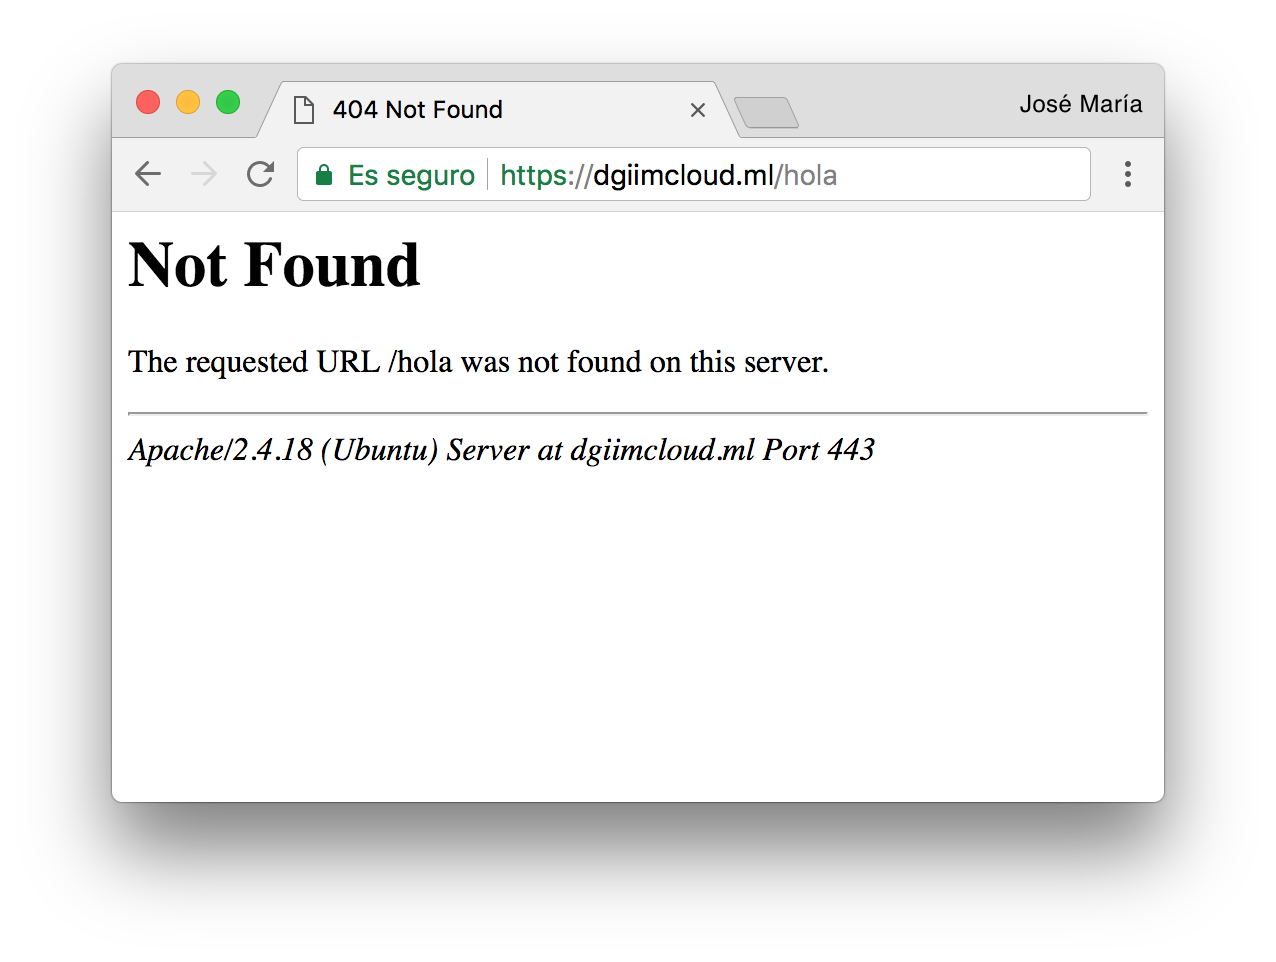
\includegraphics[width=\textwidth]{404}
\label{fig:404}
\caption{Error 404.}
\end{figure}

Hablamos en pasado pero efectivamente este sigue siendo un problema en la actualidad. No es raro entrar en algún enlace y encotrarnos con el error que podemos ver en la figura \ref{fig:404}. Incluso si no conoces la especificación del protocolo HTTP es probable que ya sepas que 404 es el código de error que nos indica que no hay nada que ver en una dirección.

La desaparición de enlaces (o \textit{link rot} en inglés) es mucho más habitual de lo que se pueda pensar. El creador de \href{pinboard.in}{Pinboard}, Maciej Cegłowski, estima que alrededor del 5\% de los enlaces que almacenan los usuarios en este servicio dejan de funcionar cada año\cite{pinboard-dead-links}. Añade además que uno de sus clientes ha visto cómo dejaban de funcionar el 90\% de los enlaces que llevaba almacenados desde 1997. En 2014, un estudio de Jonathan Zittrain, Kendra Albert y Lawrence Lessig de la Harvard Law School concluyó que aproximadamente el 50\% de los enlaces que aparecen en resoluciones del Tribunal Supremo de los Estados Unidos ya no redireccionan a la información original\cite{scotus-dead-links}. Por estos motivos existen servicios como \href{https://archive.org/}{The Internet Archive}, que se dedica a guardar copias de las páginas web para preservarlas de cara al futuro, o el propio Pinboard, que ofrece a sus usuarios la posibilidad de almacenar copias de los artículos que añadan al servicio.

% subsection fragilidad (end)

\subsection{Hipercentralización} % (fold)
\label{sub:hipercentralización}

En la \textit{Declaración de Independencia del Ciberespacio}\cite{cyberspace-independence} John Perry Barlow describía una utopía digital en la que los ciudadanos de la red se autogobiernan y las antiguas instituciones no tienen nada que hacer. ``De parte del futuro, os pido a vosotros del pasado que nos dejéis en paz. No sois bienvenidos entre nosotros. No tenéis la soberanía del lugar donde nos reunimos.'' 

Por desgracia, esta no es la realidad en el año 2017. En la actualidad la web está altamente centralizada. La práctica totalidad de los usuarios de Internet dependen de una serie de servicios concretos. Por poner algunos ejemlos, en 2015 Facebook anunció que más de mil millones de usuarios utilizaron el servicio en un mismo día\cite{billion-facebook}, mientras que una caída del servicio de Google en 2013 provocó una reducción del tráfico de internet del 40\%\cite{google-outage}.

La \textit{hipercentralización} de la red trae consecuencias negativas. Organizaciones como la NSA sólo tienen que intervenir el tráfico de unas pocas empresas para espiarnos, tal y como revelan las filtraciones de Edward Snowden\cite{snowden-leaks}. La censura es mucho más fácil de establecer ya que sólo hay que bloquear el acceso a una serie de sitios concretos. 

% subsection hipercentralización (end)

\subsection{Ineficiencia} % (fold)
\label{sub:ineficiencia}

Para comprobar la ineficiencia de transmitir información por HTTP vamos a poner un ejemplo. El vídeo más visto de YouTube según Wikipedia a 17 de octubre de 2017 es ``Luis Fonsi - Despacito ft. Daddy Yankee''\cite{most-viewed-yt}, con 4.055.733.709 visualizaciones a las 11:47.

Supongamos que el vídeo siempre se reprodujese en 720p, de tal forma que el archivo pesa exactamente 67,1MB. 4.055.733.709 visualizaciones de un archivo de 67,1MB son 272.139.731.874MB descargados. Suponiendo que a Google le costase 1 céntimo transmitir 1GB de información (incluyendo todos los gastos del servidor), ya se habría gastado más de 
272.139.731,874€ en transmitir un único vídeo.

Este precio de 1 céntimo por GB quizás sea posible para Google pero no lo es ni mucho menos para el ciudadano medio. La tabla de precios del CDN de Amazon, CloudFront es la siguiente\cite{cloudfront-prices}:

\begin{figure}[H]
	\centering
	\texttt{
\begin{tabular}{lrrrr}
  & Estados Unidos & Europa & Japón & India\\
  Primeros 10TB/mes & 0,085USD & 0,085USD & 0,140USD & 0,170USD\\
  Siguientes 40TB/mes & 0,080USD & 0,080USD & 0,135USD & 0,130USD\\
  Siguientes 100TB/mes & 0,060USD & 0,060USD & 0,120USD & 0,110USD\\
  Siguientes 350TB/mes & 0,040USD & 0,040USD & 0,100USD & 0,100USD\\
\end{tabular}}
	\caption{Tabla de precios de Amazon CloudFront en algunas regiones.}
\end{figure}
\vspace{-.5cm}
Podemos observar fácilmente que los precios son mucho mayores, ya que además se cobran las peticiones HTTP y HTTPS. La conclusión a la que queremos llegar es que a pesar de que HTTP ha abaratado muchísimo los costes de distribución de información, siguen siendo altos. Si el contenido a distribuir se encuentra en un servidor concreto, es necesario pagar los gastos generados tanto por distribuir el contenido como por el propio mantenimiento del servidor.


% subsection ineficiencia (end)

\subsection{Dependencia} % (fold)
\label{sub:dependencia}

% subsection dependencia (end)

% section problemas_de_http (end)

\section{La web distribuida} % (fold)
\label{sec:la_web_distribuida}

\subsection{Tecnologías de web distribuida} % (fold)
\label{sub:tecnologías_de_web_distribuida}

% subsection tecnologías_de_web_distribuida (end)

% section la_web_distribuida (end)

\section{El protocolo IPFS} % (fold)
\label{sec:el_protocolo_ipfs}

\subsection{IPFS en detalle} % (fold)
\label{sub:ipfs_en_detalle}

% subsection ipfs_en_detalle (end)

\subsection{Cómo soluciona IPFS los problemas de HTTP} % (fold)
\label{sub:cómo_soluciona_ipfs_los_problemas_de_http}

% subsection cómo_soluciona_ipfs_los_problemas_de_http (end)

% section el_protocolo_ipfs (end)

\section{La web distribuida en la actualidad} % (fold)
\label{sec:la_web_distribuida_en_la_actualidad}

\subsection{La Wikipedia descentralizada} % (fold)
\label{sub:la_wikipedia_descentralizada}

% subsection la_wikipedia_descentralizada (end)

\subsection{Neocities} % (fold)
\label{sub:neocities}

% subsection neocities (end)

\subsection{La web del referéndum catalán de 2017} % (fold)
\label{sub:la_web_del_referéndum_catalán_de_2017}

% subsection la_web_del_referéndum_catalán_de_2017 (end)

% section la_web_distribuida_en_la_actualidad (end)

%----------------------------------------------------------------------------------------
%	BIBLIOGRAFÍA
%----------------------------------------------------------------------------------------

\newpage
\printbibliography
%----------------------------------------------------------------------------------------

\end{document}